% icai2017.sty uses the next packages:
% geometry, [utf8]inputenc, [T1]fontenc, [english]babel, graphicx, [intlimits]amsmath, amssymb, amsthm, caption, titlesec, url
%
% Defined theorem-like environments:
% definition, theorem, lemma, remark, example, corollary, proof
%
% You can define new theorem-like environment in the following way (see amsthm.sty):
% \newtheorem{prob}[theorem]{Problem}

\documentclass{article}
\usepackage{icai2017}
\usepackage{graphicx}

\usepackage{array}
\newcolumntype{L}[1]{>{\raggedright\let\newline\\\arraybackslash\hspace{0pt}}m{#1}}
\newcolumntype{C}[1]{>{\centering\let\newline\\\arraybackslash\hspace{0pt}}m{#1}}
\newcolumntype{R}[1]{>{\raggedleft\let\newline\\\arraybackslash\hspace{0pt}}m{#1}}

\newtheorem{prob}[theorem]{Problem}

\title{Cross Translational Unit Analisys in Clang Static Analyzer: Prototype and measurements}
\author{D\'aniel Krupp\inst1, Zolt\'an Porkol\'ab\inst1,Gy\"orgy Orb\'an\inst1\\ 
        G\'abor Horv\'ath\inst2, Zolt\'an Gera\inst2}
\institute{\inst1Ericsson Ltd., \inst2E\"{o}tv\"{o}s Lor\'{a}nd University, Faculty of Informatics\\
             \inst1\url{daniel.krupp@ericsson.com}, 
             \inst1\url{zoltan.porkolab@ericsson.com},
             \inst1\url{gyorgy.orban@ericsson.com},
             \inst2\url{xazax@caesar.elte.hu}, 
             \inst2\url{gerazo@caesar.elte.hu}}
             
\begin{document}
\maketitle

\begin{abstract}
Today Clang SA can perform (context-sensitive) inter-procedural analysis for 
C,C++ and Objective C files by ''inlining'' 
the called function into the callers context. This means that that the full 
calling context
(assumptions about function parameters, global variables) is passed when 
analyzing the called function and
then the assumptions about the returned value is passed back to the caller. 
This works well for function calls within a
translation unit (TU), but when the symbolic execution reaches a function that 
is implemented in another TU, the analyzer engine 
skips the analysis of the called function definition. In particular,
assumptions about references and pointers passed as function 
parameter get invalidated, and the return value of the function will be unknown.
Loosing precision this way may lead to false positive 
and false negative findings.

The cross translation unit (CTU) feature would allow the analysis of called 
functions even if the definition of the function is external to the currently 
analyzed TU. This would allow detection of bugs in library functions stemming
from incorrect usage (e.g. a library assumes that the user will free a memory 
  block allocated by the library), and allows for more precise analysis in 
general of the caller if a TU external function is invoked 
(by not loosing assumptions).

We implemented (based on the prototype by A. Sidorin et al. \cite{artemctu}) 
the Cross Translation Unit analysis feature for Clang SA (4.0) and evaluated 
its performance on various open source projects. In our presentation we show 
that with the CTU feature we found many new true positive reports and 
eliminated some false positives in real open source projects. We show that 
while the total analysis time increases to 2-3 times, the execution remains
scalable to the number of processors. We also point out how the analysis
coverage changes that may lead to the loss of reports compared to the 
non-CTU baseline.
\keywords C++ programming language, static analysis, cross translation unit analysis
\end{abstract}

\section{Description of the CTU prototype}
In this project we are working on a method which enables CTU analysis 
by inlining external function definitions using clang's existing ASTImporter 
(see \cite{astimporter}) functionality.
One of our goals was to have minimal, isolated, and lightweight changes.
We added less than 300 lines of code to the clang codebase 
(1200 lines of code including the support utilities that are 
  separate executables and tests). 

\subsection{ 2-pass analysis}
To perform the analysis we need to run clang on the whole source code two times 
(see Figure \ref{figctu}).\\
%[Cross Translation Analysis Overview]
\textbf{1st pass:}\\
The first analysis phase generates 3 important outputs: AST dump of all
Tranlsation units, a map file for functions with external linkage, the global call flow graph.
The AST binary (using the {\tt clang -cc1 -emit-pch}) 
of each TU is generated into a temporary directory. 
The mangled name and location of all externally linkable functions 
are collected into the function definition index (externalFnMap.txt). 
The global call graph of the program is stored in a file called (cfg.txt).
\begin{figure}[h!]
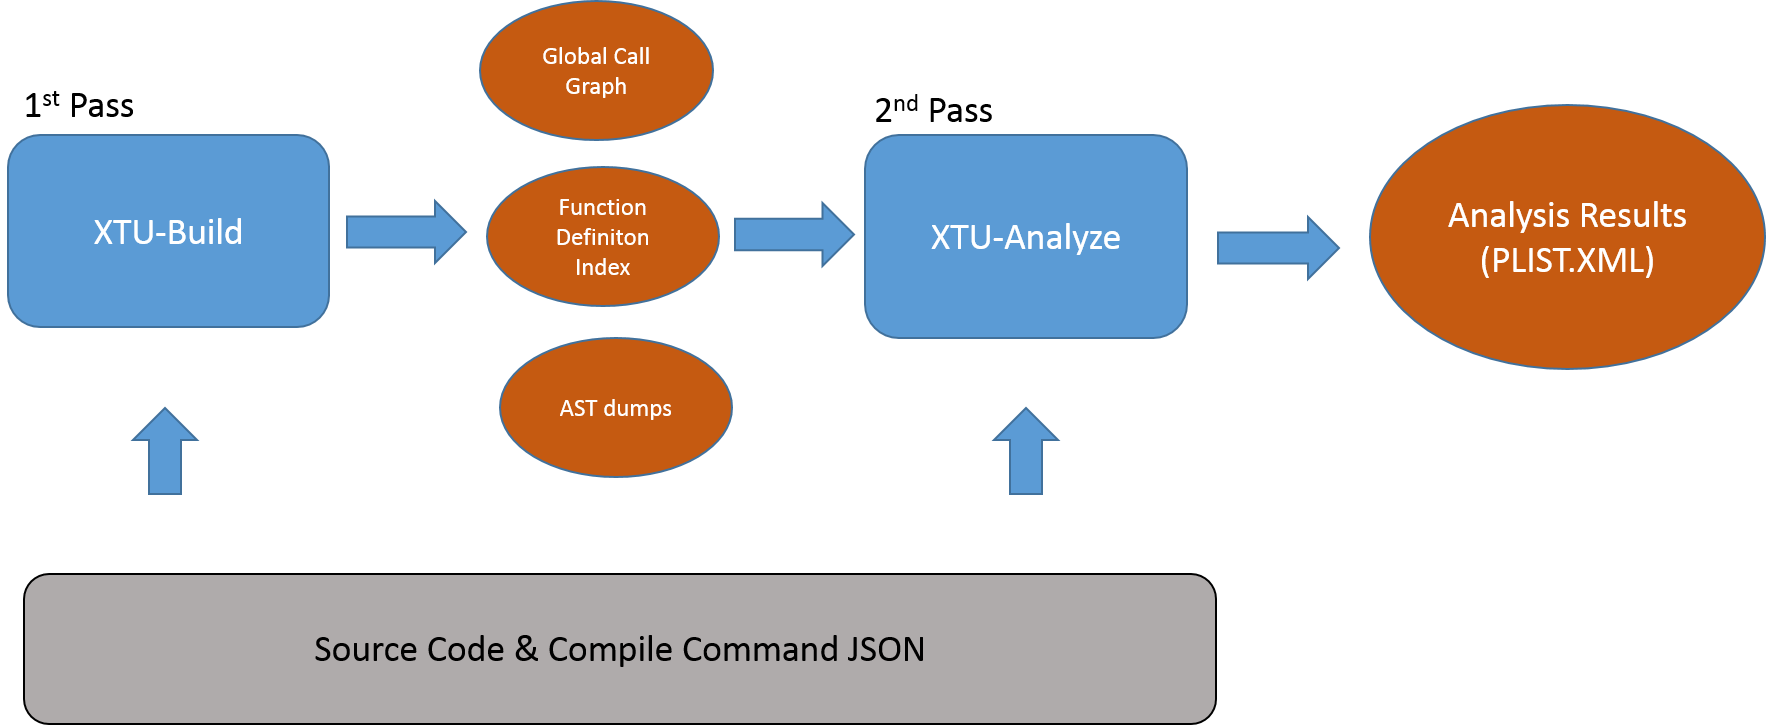
\includegraphics[width=\textwidth]{images/ctu.png}
\caption{2-Pass CTU analysis overview}
\label{figctu}
\end{figure}

\textbf{2nd pass:}\\
The Clang Static Analyzer is run for all translation units. When during the
analysis a TU external function is reached, the location of the definition 
of that function is looked up from in the function definition index and the 
definition is imported from the containing AST binary into the caller's context
using the ASTImpoter library.

\subsection{Traversal of the the control flow graph}
In the non-CTU analysis, functions that are not called from within the TU are
analyzed first as ''top-level'' functions and all functions that are 
non-top-level are only analyzed in a call context (as they are called). 
In our CTU implementation, when analyzing a source file, we start the analysis
from the same top-level functions as the original non-CTU method even if a given
function is called from another TU (according to the global CFG). 
The reason for the choice of this strategy is that if the project 
contains test cases then library functions would only be analyzed with 
the concrete test values which would result in loss of generality of the analysis. 

The source code of the prototype is available in this clang GitHub fork 
\cite{ctugithub}.


\section{ Results on Open Source projects}
We have analyzed many open source projects 
(ffmpeg, tmux, curl, vim, postgresql...) using CTU and 
found many new true positive reports (see Table \ref{tblfindings}.

The measurements were taken using clang 4.0 as the baseline and the same 
clang 4.0 with the CTU patch. Only the by default enabled (stable) checkers 
were switched on.
\begin {table}[h!]
\centering
\begin{tabular}{| L{1.6cm}| C{1.6cm} | C{1.6cm} | C{1.6cm} | C{1.6cm} | C{1.6cm} |}
  \hline
  Analyzed project& All Non-CTU Findings (baseline)&All CTU Findings&New CTU findings & Disappeared findings & Successfully / Failed to analyze
  \\
  \hline
  \hline
  FFMpeg& 339& 399 & 101& 41& 1555/8 files \\
  \hline
  TMux& 49& 77 & 29& 1 & 133/0 files \\
  \hline
  Curl& 7& 11& 4& 0 & 280/13 files\\
  \hline  
\end{tabular}
\caption{CTU and Non-CTU results comparison}
\label{tblfindings}
\end{table}

\subsection{Quality of new results} 
The new analysis found significant number of new results on all projects. 
The number of findings increased by 17\% to 50\%.
We examined the new findings in detail and most of them are true positive.
According to our evaluation the CTU analysis did not introduce any new false 
positives (there was no precision loss at CTU boundary).

The CTU analysis revealed many new bugs that require length symbolic analysis,
such as memory leak problems (unix.Malloc), dereference of null pointers 
(core.NullDereference, core.NonNullParamChecker, core.CallAndMessage)
and usage of uninitialized values (core.uninitialized.Assign,\\ 
core.uninitialized.Branch, core.UndefinedBinaryOperatorResult). 

We expected that the bug path length of the new results will be longer 
than the results in the baseline, due to the long traversal of function 
calls into external source files (see Table \ref{tblbpl}. This assumption turned out to be true as 
the median of the bug path length of new bugs is 16 compared to the non-ctu 
case 7 (for ffmpeg). However in practice 16 long bug path are still 
manageable for programmers.

\begin {table}[h!]
\centering
\begin{tabular}{| C{2cm}|| C{2cm} | C{2cm} |C{2cm} |C{2cm} |}
  \hline
  Analyzed project & Median of bug path length (BPL) in baseline&Median of BPL CTU&Median of BPL of new findings&Median of BPL of disappeared findings\\
  \hline
  \hline
  FFMpeg&7&9&16&14\\
  \hline
  TMux&16&16&17&6\\
  \hline
  Curl& 1&1&12&n.a.\\
  \hline  
\end{tabular}
\caption{CTU and Non-CTU Bug Path Length comparison}
\label{tblbpl}
\end{table}

Some of the results disappeared compared to the baseline analysis. 
We are still investigating the reason for this, but we primarily 
suspect two reasons:

1. The coverage of the analysis somewhat changed for the base file 
analyzed, because in some cases the analysis node budget is consumed by 
the traversal of long CTU paths instead of paths inside the base file. 
It must be noted that in the Non-CTU case the paths inside the base file 
have inherently imprecise assumptions about external functions.

2. It is also possible that some of the findings disappeared 
compared the baseline because they were false positives as they were based on 
false assumptions about unknown external functions. However we think this is to a 
less extent as Clang SA checkers are written conservatively to report less 
false positives.

Detailed analysis of the results can be found in the following pages: 
\cite{ffmpegres}, \cite{curlres},\cite{tmuxres}.

\subsection{Performance}
In general the analysis time (including both analysis passes) 
increased ~2 to ~2.5 times the baseline non-CTU analysis time on all analyzed
projects (see Table \ref{tbltime}). The increment is due to the first analysis phase and the extra effort
of loading the definition of external function from the disc during the
analysis. The measurements were performed on the same machine, on 16 CPU cores.
The resource need of the new analysis is not dramatic and the solution is
similarly scalable to multiple CPUs as the baseline, as all build actions
are analyzed independently.

\begin {table}[h!]
\centering
\begin{tabular}{| L{2cm}| C{2cm} | C{2cm} | C{2cm}|}
  \hline
  Analyzed project& Analysis Time (baseline)[s]&Analysis Time XTU (1st + 2nd Phase)[s]\\
  \hline
  \hline
  FFMpeg& 318&44+693\\
  \hline
  TMux& 39&4+75\\
  \hline
  Curl& 32&6.5+54\\
  \hline  
\end{tabular}
\caption{CTU and Non-CTU analysis time comparison}
\label{tbltime}
\end{table}

\section{Future work}

\begin{itemize}
\item The current CTU prototype is usable only for C projects. 
We experienced many crashes and asserts with the ASTImporter for C++ projects. 
ASTImporter needs to be improved to handle C++ language constructs better.
\item Do we lose true positives and coverage in the base file. 
We plan to measure coverage and experiment with different strategies
to build the exploded graph. One simple strategy might be to bound
the number of file traversals.
\item Flow based bug reports have a so-called uniqueing location that helps
to differentiate them. This works for single TUs, but we would like
to extend this to multiple TUs.
\item During the analysis, we need to store the dumped ASTs temporarily. 
We thought of ways decrease the disc allocation by compressing or 
more efficiently storing the AST dumps.
\end{itemize}

\section{Credits}
This work is based on earlier work of Aleksei Sidorin , Artem Dergachev 
et al. See \url{http://lists.llvm.org/pipermail/cfe-dev/2015-October/045730.html}

\section{ References}
\begin{thebibliography}{9}
\bibitem{ccelte} Cross-TU Analysis results on open source projects: http://cc.elte.hu/

\bibitem{artemctu} Artem Dergachev, Aleksei Sidorin Cross TU Analysis for Clang 
3.4 \url{http://lists.llvm.org/pipermail/cfe-dev/2015-October/045730.html}

\bibitem{ericssonctu} Ericsson CTU open source repository: \url{https://github.com/dkrupp/clang/tree/ctu-master}
\bibitem{ctugithub} \url{https://github.com/dkrupp/clang/tree/ctu-master}
\bibitem{ffmpeg} FFMPeg project,  \url{https://github.com/FFmpeg/FFmpeg}
\bibitem{tmux} TMux project, \url{https://github.com/tmux/tmux}
\bibitem{curl} CUrl project, \url{https://github.com/curl/curl}
\bibitem{astimporter} ASTImporter, \url{http://clang.llvm.org/doxygen/classclang_1_1ASTImporter.html}
\bibitem{ffmpegres} FFmpeg CTU Results {\small \url{https://github.com/dkrupp/clang/wiki/FFMpeg-XTU-Analysis}}
\bibitem{tmuxres} TMUX CTU Results \url{https://github.com/dkrupp/clang/wiki/TMUX-XTU-Analysis}
\bibitem{curlres} CURL CTU Results \url{https://github.com/dkrupp/clang/wiki/Curl-XTU-Analysis}
\end{thebibliography}
\end{document} 
